\documentclass[12pt, twoside]{article}
\usepackage[letterpaper, margin=1in, headsep=0.5in]{geometry}
\usepackage[english]{babel}
\usepackage[utf8]{inputenc}
\usepackage{amsmath}
\usepackage{amsfonts}
\usepackage{amssymb}
\usepackage{tikz}

\usepackage{pgfplots}
\pgfplotsset{width=9cm,compat=1.9}

\usepackage{venndiagram}

\usepackage{graphicx}
\usepackage{enumitem}
\usepackage{multicol}

\usepackage{fancyhdr}
\pagestyle{fancy}
\fancyhf{}
\renewcommand{\headrulewidth}{0pt} % disable the underline of the header

\fancyhead[LE]{\thepage}
\fancyhead[RO]{\thepage \\ Name: \hspace{4cm} \,\\}
\fancyhead[LO]{BECA / Dr. Huson / IB Mathematics\\* Unit 4: Linear functions and regression\\* 16 January 2020}

\begin{document}
\begin{enumerate}
    \subsubsection*{4.10 Do Now: Quadratics, function operations, linear equations}
    \item {[Maximum mark: 6]} \\[0.3cm]
    The diagram shows part of the graph of the quadratic function $f$. 
         \begin{center}
         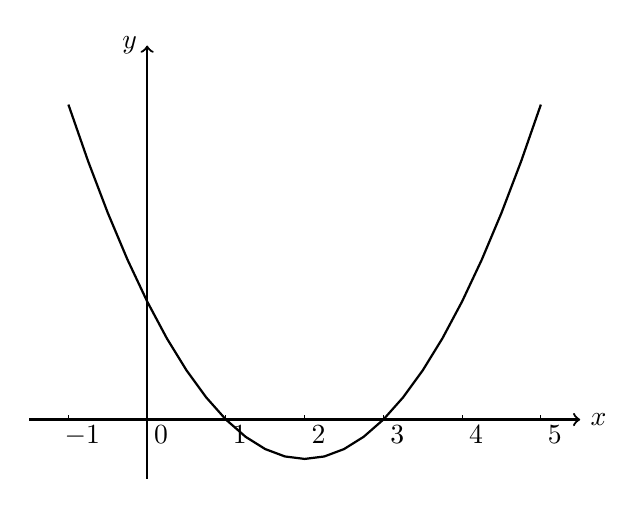
\begin{tikzpicture}[xscale=1.0, yscale=0.5]
                 %\draw [thin, color=gray, xstep=1.0cm,ystep=1.0cm] (-3.5,-3.5) grid (3.5,3.5);
                 %\draw [thin, color=lightgray,, xstep=0.2cm,ystep=0.2cm] (-5.5,-4.5) grid (5.5,6.5);
                 \foreach \x in {-1, 0,1,2,3, 4, 5}
                     \draw[shift={(\x,0)},color=black] (0pt,-1pt) -- (0pt,3pt) node[below]  {$\quad \x$};
                 %\foreach \y in {-3, -2,-1,0,1,2,3}
                     %\draw[shift={(0,\y)},color=black] (2pt,0pt) -- (-2pt,0pt) node[left]  {$\y$};
                 \draw [thick, ->] (-1.5,0) -- (+5.5,0) node [right] {$x$};
                 \draw [thick, ->] (0,-1.5) -- (0,9.5) node [left] {$y$};
             \draw [thick] plot[domain= -1:5] (\x, {(\x-2)^2 -1});
             %\draw [thick] plot[domain= -1:2] (\x, \x*1/2 -2);
             %\draw [thick] (-2,-2).. controls (0,-1) and (2,0) .. (3,1);
             %\draw [fill] (-3,3) circle[radius=0.1] node[above left]{$A(-3,3)$};
         \end{tikzpicture}
         \end{center}
         The vertex is at $(2, -1)$ and the $x$-intercepts are at 1 and 3.\\[0.25cm]
         The function $f$ can be written in the form $f(x)=(x-h)^2+k$.
         \begin{enumerate}%[itemsep=2cm]
             \item Write down the value of $h$ and $k$. \hfill [2]\\[0.25cm]
             The function can also be written in the form $f(x)=(x-a)(x-b)$.
             \item Write down the value of $a$ and $b$. \hfill [2]
             \item Find the $y$-intercept. \hfill [2]
         \end{enumerate}
         \begin{tikzpicture}
             \draw (0,2) rectangle (15.5,11);
             \draw [dotted] (1,10)--(14,10);
             \draw [dotted] (1,9)--(14,9);
             \draw [dotted] (1,8)--(14,8);
             \draw [dotted] (1,7)--(14,7);
             \draw [dotted] (1,6)--(14,6);
         \end{tikzpicture}

\newpage
    \item {[Maximum mark: 6]} \\[0.3cm]
    The diagram below shows the graph of a function $f$ for $-\frac{5}{2} \leq x \leq 3$. 
         \begin{center}
         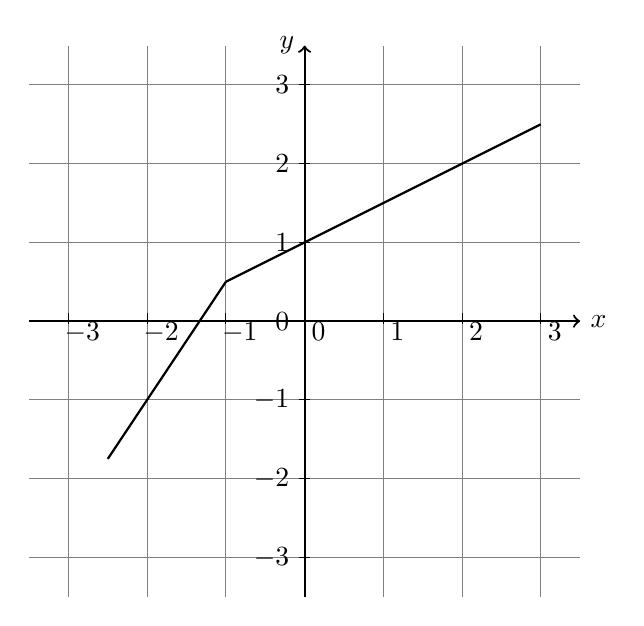
\begin{tikzpicture}[scale=1.0]
                 \draw [thin, color=gray, xstep=1.0cm,ystep=1.0cm] (-3.5,-3.5) grid (3.5,3.5);
                 %\draw [thin, color=lightgray,, xstep=0.2cm,ystep=0.2cm] (-5.5,-4.5) grid (5.5,6.5);
                 \foreach \x in {-3, -2, -1, 0,1,2,3}
                     \draw[shift={(\x,0)},color=black] (0pt,-1pt) -- (0pt,3pt) node[below]  {$\quad \x$};
                 \foreach \y in {-3, -2,-1,0,1,2,3}
                     \draw[shift={(0,\y)},color=black] (2pt,0pt) -- (-2pt,0pt) node[left]  {$\y$};
                 \draw [thick, ->] (-3.5,0) -- (+3.5,0) node [right] {$x$};
                 \draw [thick, ->] (0,-3.5) -- (0,3.5) node [left] {$y$};
             \draw [thick] (-1,0.5)--(3,2.5);
             \draw [thick] (-1,0.5)--(-2.5,-1.75);
             %\draw [thick] plot[domain= -1:2] (\x, \x*1/2 -2);
             %\draw [thick] (-2,-2).. controls (0,-1) and (2,0) .. (3,1);
             %\draw [fill] (-3,3) circle[radius=0.1] node[above left]{$A(-3,3)$};
         \end{tikzpicture}
         \end{center}
         \begin{enumerate}%[itemsep=2cm]
             \item Write down the value of $f(-2)$. \hfill [1]
             \item Write down the value of $f^{-1}(1)$. \hfill [2]
             \item Sketch the graph of $f^{-1}$ on the grid. \hfill [3]
         \end{enumerate}
         \begin{tikzpicture}
             \draw (0,1) rectangle (15.5,11);
             \draw [dotted] (1,10)--(14,10);
             \draw [dotted] (1,9)--(14,9);
             \draw [dotted] (1,8)--(14,8);
             \draw [dotted] (1,7)--(14,7);
             \draw [dotted] (1,6)--(14,6);
         \end{tikzpicture}

\newpage 
    \item {[Maximum mark: 5]} \\[0.3cm]
    The diagram shows the straight line $L_1$, which intersects the $x$-axis at $A(j, 0)$ and the $y$-axis at $B(0,k)$.
        \begin{center}
            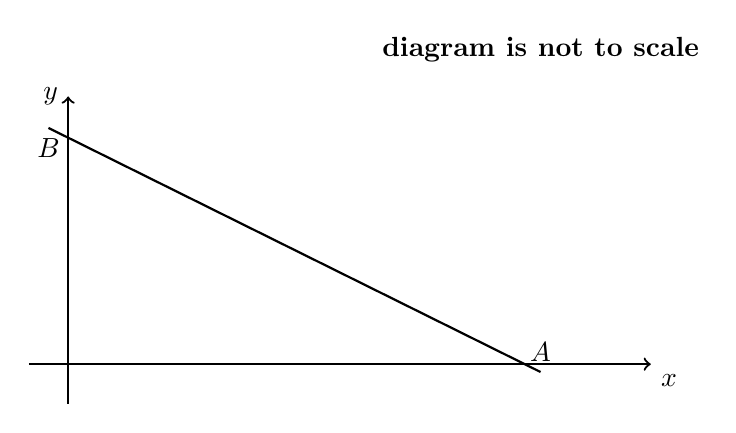
\begin{tikzpicture}[scale=1]
            %\draw [help lines] (0,0) grid (10,8);
            \draw [thick, ->] (-0.5,0) -- (7.4,0) node [below right] {$x$};
            \draw [thick, ->] (0,-0.5)--(0,3.4) node [left] {$y$};
            %\draw [fill] (9,5) circle [radius=0.1];
            \draw [thick, -] (-0.25,3) node [below] {$B$}--(6,-0.1) node [above] {$A$};
            \node at (6,4){\textbf{diagram is not to scale}};
            \end{tikzpicture}
        \end{center}
        The equation of $L_1$ is $\displaystyle y=-\frac{2}{5}x+3$.
        \begin{enumerate}%[itemsep=3cm]
            \item Find the value of \hfill [2]
                \begin{enumerate}
                    \item $j$
                    \item $k$
                \end{enumerate}
            \item The line $L_2$ is perpendicular to $L_1$ and passes through $(4,3)$.
                \begin{enumerate}
                    \item Write down the gradient for the line $L_2$. \hfill [1]
                    \item Hence, write down the equation of $L_2$. Leave your answer in the form \\ $y-a=m(x-b)$. \hfill [2]
                \end{enumerate}
        \end{enumerate}
        \begin{tikzpicture}
            \draw (0,3) rectangle (15.5,11);
            \draw [dotted] (1,10)--(14,10);
            \draw [dotted] (1,9)--(14,9);
            \draw [dotted] (1,8)--(14,8);
            \draw [dotted] (1,7)--(14,7);
        \end{tikzpicture}

\newpage 
    \item {[Maximum mark: 5]} \\[0.3cm]
    Let $f(x)=x+3$ and $g(x)=x^2$, for $x \in R$.
        \begin{enumerate}
            \item Find $x$ such that $f(x)=0$. \hfill [1]
            \item Find $(f \div g)(1)$. \hfill [1]
            \item Find $(g \circ f)(x)$. \hfill [1]
            \item Find $f^{-1}(7)$. \hfill [2]
        \end{enumerate}
        \begin{tikzpicture}
            \draw (0,-4) rectangle (15.5,11);
            \draw [dotted] (1,10)--(14,10);
            \draw [dotted] (1,9)--(14,9);
            \draw [dotted] (1,8)--(14,8);
            \draw [dotted] (1,7)--(14,7);
            \draw [dotted] (1,6)--(14,6);
        \end{tikzpicture}

\end{enumerate}
\end{document}